% https://tex.stackexchange.com/a/297685/173708
% modified, commented
\documentclass{standalone}
\usepackage{tikz}
\usetikzlibrary{arrows.meta,positioning}

\begin{document}

% remove subsection
% remove /begin{center}

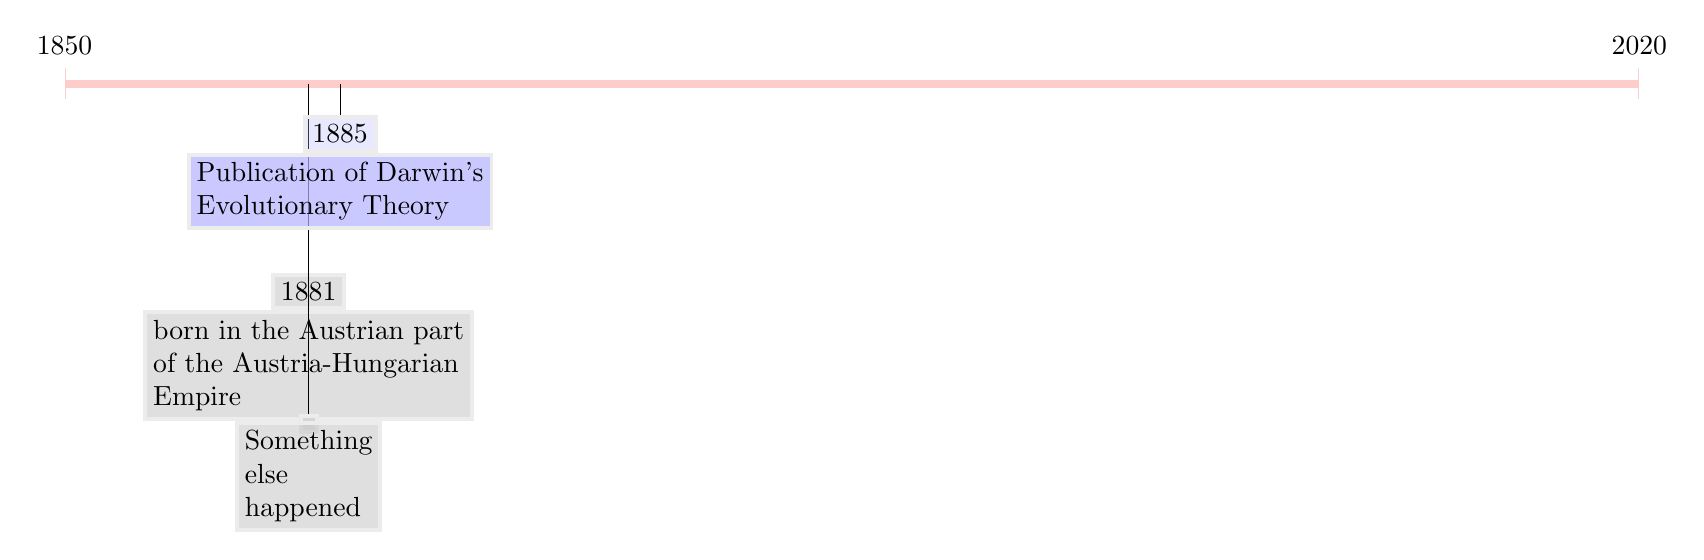
\begin{tikzpicture}[node distance = 0mm,
	TN/.style args = {#1/#2}{% as Transparency Node
	    fill=#1,
	    fill opacity=#2,
	    text opacity=1, 
	    align=flush left,
	    inner sep=1mm, 
	    outer sep=0.25mm, 
	    draw=gray!15,
	    line width=0.5mm,
	    below},	        
    TN/.default = gray!50/0.5,
	L/.style = {% as Line
	    draw=red!20, 
	    line width=1mm,
	    {Bar[width=4mm,line width=0.4pt]}-{Bar[width=4mm,line width=0.4pt]}
        }
    ]
    
	\draw[L]    ( 0,0)  coordinate (s)
	                    node[above=2mm] {1850} -- + 
	            (20,0)  node[above=2mm] {2020};
	            
	\draw (3.1,0) -- + (0,-2.4)
	        node (e1)   [TN]              {1881}
	        node (e1a)  [TN,below=of e1]  {born in the Austrian part\\
	                                       of the Austria-Hungarian\\
	                                       Empire};

	\draw (3.1,0) -- + (0,-4.2)
	        node (e1y)   [TN]              {}
	        node (e1t)  [TN,below=of e1a]  {Something\\
	                                       else\\
	                                       happened};
	                                       
	                                       
	\draw (3.5,0) -- + (0,-0.4) 
	        node (e2)   [TN=blue!30/0.3]  {1885}
	        node (e2a)  [TN=blue!30/0.7,
	                     below=of e2]    {Publication of Darwin's\\
	                                      Evolutionary Theory};
\end{tikzpicture}

\end{document}